%! TEX root = ./main.tex

\section{Transport Layer}
\begin{itemize}
    \item Link between network and application layer
        \begin{itemize}
            \item Network is best-effort
                \begin{itemize}
                    \item Packages can get:
                        \begin{itemize}
                            \item Lost
                            \item Corrupted
                            \item Reordered
                            \item Delayed
                            \item Duplicated
                        \end{itemize}
                \end{itemize}
            \item Applications should be restricted to app-specific functionality
            \item Transport layer is key
        \end{itemize}
    \item Requirements
        \begin{itemize}
            \item Data delivery to the correct application
                \begin{itemize}
                    \item Demultiplexing required
                \end{itemize}
            \item File or byte-stream abstraction for applications
            \item Reliability
            \item No overload of receiver or network
        \end{itemize}
\end{itemize}

\subsection{Reliable Transport}
\begin{itemize}
    \item Key properties
        \begin{itemize}
            \ides{Correctness:} Input is equal output
                \begin{itemize}
                    \ides{Formal Definition:} A packet is always resent if the previous packet was lost or corrupted. A packet may be resent at other times.
                \end{itemize}
            \ides{Timeliness:} Minimize time between input and output
            \ides{Efficiency:} Minimize use of bandwidth
            \ides{Fairness:} Respect other players
        \end{itemize}
\end{itemize}

\subsubsection{Protocol}
\begin{itemize}
    \item Incrementally build up a reliable transmission protocol
    \ides{Lossy Channel}
        \begin{itemize}
            \ides{Goal:} Lossless transmission
            \item
\begin{verbatim}
# Sender side
for word in list:
    send_packet(word)
    set_timer()

    upon timer going off:
        if no ACK received:
            send_packet(word)
            reset_timer()
    upon ACK:
        pass

# Receiver Side
receive_packet(p)
if check(p.payload) == p.checksum:
    send_ack()

    # Send word to application if not already done
    if word not delivered:
        deliver_word(word)

else:
    pass

\end{verbatim}
            \item Timer determines when packet is lost
            \ides{Timeout:} Difficult to set
                \begin{itemize}
                    \ides{Short:} Unnecessary retransmissions
                    \ides{Long:} Slow transmission
                        \begin{itemize}
                            \item Long wait for missing packets
                        \end{itemize}
                    \item Tradeoff between timeliness and efficiency
                \end{itemize}
            \ipro Is correct
            \icon Sends $1$ packet per RTT
        \end{itemize}
    \ides{Improve Timeliness}
        \begin{itemize}
            \ides{Goal:} Improve timeliness and efficiency
            \item Send multiple packets at the same time
            \item Add sequence number to each packet
            \item Add buffers to sender and receiver:
                \begin{itemize}
                    \ides{Sender:} Store packets send but not acknowledged
                        \begin{itemize}
                            \item Delete once acknowledged
                        \end{itemize}
                    \ides{Receiver:} Store out-of-sequence packets received
                        \begin{itemize}
                            \item Delete once in order and delivered
                        \end{itemize}
                \end{itemize}
            \ipro Sends multiple packets per RTT
            \icon Sender can easily overwhelm receiver
                \begin{itemize}
                    \item By sending too many packets
                \end{itemize}
        \end{itemize}
    \ides{Flow and Congestion Control}
        \begin{itemize}
            \ides{Goal:} Prevent overwhelmingness of receiver and of network
            \ides{Sliding Window:} Restrict the sender and receiver buffer to a certain size
            \ides{Sending Window:} List of sequence numbers the sender is allowed to send
                \begin{itemize}
                    \item Move forward iff the lowest packet number in the windows was acknowledged
                    \ides{Congestion Control:} Prevent overwhelming network
                \end{itemize}
            \ides{Receiving Window:} List of sequence numbers the receiver is allowed to receive
                \begin{itemize}
                    \item If lowest packet number in the window is received:
                        \begin{itemize}
                            \item Send acknowledgement for that packet
                            \item Move sending window forward
                        \end{itemize}
                    \ides{Flow Control:} Prevent overwhelming receiver
                \end{itemize}
            \item \verb+size(sending window) <= size(receiving windows)+
            \item Window size is exchanged during handshake
            \ides{Bandwidth-Delay-Product:} Window size should be $\text{Bandwidth} \cdot \text{RTT}$
                \begin{itemize}
                    \item Send so many packets that we stop sending right before receiving the first acknowledgement
                    \item Maximizes timeliness
                \end{itemize}
        \end{itemize}
    \ides{Improve ACKs}
        \begin{itemize}
            \item Efficiency is fully determined by the acknowledgement and how to handle losses
            \item Different algorithms
            \ides{Individual ACKs}
                \begin{itemize}
                    \item Acknowledge every single packet received
                    \item Losses are indicated implicitly by the missing ACK for that number
                    \item Resend missing packet after $k$ subsequent ACKs of other packets
                    \ipro \textbf{Known Fate:} We have feedback for every single packet
                    \ipro Simple algorithm
                    \ipro Not sensitive to reordering
                    \icon Loss of a ACK packet causes retransmission of that packet
                \end{itemize}
            \ides{Cumulative ACKs}
                \begin{itemize}
                    \item Acknowledge each packet but send the highest sequence number for which all previous packets were received
                    \icon Not obvious which packets were lost
                        \begin{itemize}
                            \item Duplicate ACKs (same sequence number acknowledged) is a sign of loss
                            \item We know some packets were delivered but not which one
                            \item We do not know which packet to retransmit
                        \end{itemize}
                \end{itemize}
            \ides{Full Information ACKs}
                \begin{itemize}
                    \item Combine individual and commutative ACKs
                        \begin{itemize}
                            \item I.e. say up to which were all received in-order and which were received out of order
                        \end{itemize}
                    \ipro Complete information
                    \icon Overhead
                        \begin{itemize}
                            \item When large of gaps in the receiver window
                            \item Lower efficiency
                        \end{itemize}
                \end{itemize}
        \end{itemize}
    \ides{Fairness}
        \begin{itemize}
            \item How is fairness defined?
            \item Fairness and efficiency do not always play along
            \item Give users with small demand what they want and distribute the rest evenly
            \ides{Max-Min Fair Allocation:} maximize lowest demand, then second lowest, etc.
                \begin{itemize}
                    \item Algorithm
                        \begin{enumerate}
                            \item Start with all flows at $0$
                            \item Increase all flows till there is a new bottleneck
                            \item Hold the rate of the flows which are bottlenecked
                            \item Repeat from step 2 for the remaining flows
                        \end{enumerate}
                    \item We do not know the available bandwidth in practice
                    \item Approximate it by repeatedly increasing window size and decreasing if upon a loss
                        \begin{itemize}
                            \item Loss is sign of congestion
                        \end{itemize}
                \end{itemize}
        \end{itemize}
    \ides{Regard corruption, reordering, delays, duplicates}
        \begin{itemize}
            \ides{Corruption}
                \begin{itemize}
                    \item Rely on checksum
                    \item Treat corrupted packets as lost
                \end{itemize}
            \ides{Reordering}
                \begin{itemize}
                    \item Creates duplicate ACKs
                    \item Depends on applies ACKing mechanism
                    \item Only a problem for commutative ACKs
                        \begin{itemize}
                            \item Sender may think that the packet was lost and resends
                        \end{itemize}
                \end{itemize}
            \ides{Delays}
                \begin{itemize}
                    \item Creates timeouts
                    \item Cannot be fixed
                \end{itemize}
            \ides{Duplication:}
                \begin{itemize}
                    \item May me detected by the receiver
                    \item Created duplicate ACKs
                    \item Depends on applied ACKing machanism
                    \item Only a problem for commutative ACKs
                        \begin{itemize}
                            \item Sender may think that the packet was lost and resends
                        \end{itemize}
                \end{itemize}
        \end{itemize}
\end{itemize}

\subsubsection{Example Protocols}
\begin{itemize}
    \ides{Go-Back-N (GBN)}
        \begin{itemize}
            \item Sliding window protocol
            \item Uses cumulative ACKs
            \ides{Goal:} Receiver should be as simple as possible
            \ides{Receiver}
                \begin{itemize}
                    \item Delivers packets in-order to the application
                    \item Uses commutative ACKss
                \end{itemize}
            \ides{Sender}
                \begin{itemize}
                    \item Uses a single timer to detect loss
                        \begin{itemize}
                            \item Is reset at each ACK
                        \end{itemize}
                    \item Upon timeout, resent the whole window starting with the lost one
                \end{itemize}
        \end{itemize}
    \ides{Selective Repeat (SR)}
        \begin{itemize}
            \item Sliding window protocol
            \item Uses individual ACKs
            \item Tries to avoid unnecessary retransmissions
            \ides{Receiver}
                \begin{itemize}
                    \item Uses individual ACKs
                \end{itemize}
            \ides{Sender}
                \begin{itemize}
                    \item Uses a per-packet timer to detect loss
                    \item Upon timeout, resent the lost packet
                \end{itemize}
        \end{itemize}
\end{itemize}

\subsection{Internet's Transport}
\begin{itemize}
    \item Two main protocols
    \item
        \begin{tabular}{p{0.3 \textwidth} | p{0.3 \textwidth} | l}
            Property & TCP & UDP\\
            \hline
            Data delivery to the correct application & Demultiplexing using port & Demultiplexing using port\\
            \hline
            File or byte-stream abstraction for applications & Segmentation and reassembly & NO\\
            \hline
            Reliability & ACKs and checksums & (optionally) checksums\\
            \hline
            No overload of receiver & Flow control via receiver window & NO\\
            \hline
            No overload of network & Congestion control via sender window & NO
        \end{tabular}
    \item Do not (necessarily) provide
        \begin{itemize}
            \item Delay and/or bandwidth guarantees
                \begin{itemize}
                    \item Would required changes at IP level
                \end{itemize}
            \item Sessions that survive change-of-IP-address
        \end{itemize}
\end{itemize}

\subsubsection{User Datagram Protocol (UDP)}
\begin{itemize}
    \item Unreliable, connection less, out-of-order data transfer protocol
    \item Simple extension of IP
    \ides{Header}
        \begin{itemize}
            \item $4$ header fields
            \ides{SRC Port:} Port of destination
            \ides{DST Port:} Port of source
            \ides{Checksum:} Checksum calculated over data and pseudoheader
            \ides{Length:} Size of the data section
        \end{itemize}
    \ides{Data Section:}
        \begin{itemize}
            \item Variable length
        \end{itemize}
    \ipro No delay of connection establishment
    \ipro No delay for ordering and reliable delivery
    \ipro Small packet overhead
        \begin{itemize}
            \item Due to small header
        \end{itemize}
    \ipro Better scalability
        \begin{itemize}
            \item Due to no state, buffer and timer
        \end{itemize}
    \ipro Send data right away
        \begin{itemize}
            \item No flow and congestion control
            \item Just send it
        \end{itemize}
    \ides{Halve-Duplex:} One-way channel
\end{itemize}

\subsubsection{Transmission Control Protocol (TCP)}
\begin{itemize}
    \item Connection-oriented, reliable, in-order byte-stream transport protocol
    \item Connection / session is a single bytestream
        \begin{itemize}
            \item State is stored in host and not network
        \end{itemize}
    \item Design
        \begin{itemize}
            \ides{ACKs:}
                \begin{itemize}
                    \item Sequence number for each byte of the payload
                    \item Cumulative ACKs
                \end{itemize}
            \ides{Checksum:} On data and pseudoheader
            \ides{Timer:}
                \begin{itemize}
                    \item Resent on timeout
                    \item Exponential backoff
                \end{itemize}
            \ides{Fast Retransmit:}
                \begin{itemize}
                    \item Retransmit packet on $3$ successive duplicate ACKs
                    \item Assume packet is lost without waiting for timer
                \end{itemize}
            \ides{Flow control}
                \begin{itemize}
                    \item Sliding window of size no larger than receiver wants
                \end{itemize}
                \ides{Congestion control}
                \begin{itemize}
                    \item Dynamic adaption to network paths's capacity
                \end{itemize}
        \end{itemize}
    \ides{Full Duplex:} Two-way channel
\end{itemize}

\paragraph{Structure}
\begin{itemize}
    \ides{Header}
        \begin{itemize}
            \item $\ge 20$ Bytes
                \begin{itemize}
                    \item At least $5$ lines
                    \item Each line is $4$ bytes long
                \end{itemize}
            \ides{SRC Port:} Port of destination
            \ides{DST Port:} Port of source
            \ides{Sequence Number:} Starting byte offset of the data sent in this segment
            \ides{Acknowledgment:} Next expected byte
            \ides{HdrLen:} Number of lines in header (for optional options)
            \ides{Must Be Zero:} has always to be $0$
            \ides{Flags:} One or multiple of \textit{SYN}, \textit{ACK}, \textit{FIN}, \textit{RST}, \textit{PSH}, \textit{URG}
            \ides{Advertised Window:} Window size of the receiver
            \ides{Checksum:} Checksum calculated over data and pseudoheader
            \ides{Urgent Pointer:} Mark data urgent
            \ides{Options:}
                \begin{itemize}
                    \item Additional options
                    \item Variable size
                \end{itemize}
        \end{itemize}
    \ides{Data Section}
        \begin{itemize}
            \item Called TCP segment
            \item Contains multiple consecutive bytes of the byte stream
            \item Variable length $\le \text{MSS}$
                \begin{itemize}
                    \ides{Maximum Transmission Unit (MTU):} Maximal size of a IP packet
                    \item TCP packet consists of $\ge 20$ Bytes header $+$ segment
                        \ides{Maximum Segment Size (MSS)} $= \text{MTU} - (\text{IP header}) - (\text{TCP header})$
                \end{itemize}
            \item Take $\le n$ bytes from the byte stream and put them in one segment
        \end{itemize}
    \item Packet send, when one of:
        \begin{itemize}
            \item Segment full
            \item Timer times out
                \begin{itemize}
                    \item Different timer from the ACK timer
                \end{itemize}
        \end{itemize}
    \ides{Sequence Number and ACKing}
        \begin{itemize}
            \ides{Initial Sequence Number (ISN):} Number of the first byte to send
                \begin{itemize}
                    \item Chosen at random
                        \begin{itemize}
                            \item For security reason
                            \item Prevent confusion of packets when reusing ports
                        \end{itemize}
                \end{itemize}
            \item Sliding window starts at $\text{ISN} + i$
            \item Receiver ACKs last $+ 1$ byte received in order
                \begin{itemize}
                    \item I.e. the next byte it expects
                    \item May send duplicate ACKs
                \end{itemize}
        \end{itemize}
    \ides{Flow Control}
        \begin{itemize}
            \ides{Advertised Windows W:} Number of bytes the sender can send starting at the next expected byte
            \item \verb+size(receiver window) >= W+
            \item At most W bytes can be in flight
            \item Transfer speed $= \min \{B, \frac{W}{\text{RTT}}\}$
                \begin{itemize}
                    \ides{Windows Size W} in bytes and constant
                    \ides{RTT} in seconds and constant
                    \ides{Bandwidth B} in bytes/second
                \end{itemize}
        \end{itemize}
\end{itemize}

\paragraph{Connection}
\begin{itemize}
    \ides{Establishment}
        \begin{itemize}
            \ides{3-Way Handshake:}
                \begin{itemize}
                    \item A picks ISN at random
                    \item A sends packet
                        \begin{itemize}
                            \item Set sequence number to A's chosen ISN
                            \item Set flag to \textit{SYN} (synchronize sequence number)
                        \end{itemize}
                    \item B picks ISN at random upon receiving packet from A
                    \item B sends packet
                        \begin{itemize}
                            \item Set sequence number to B's chosen ISN
                            \item Set acknowledged to A's ISN $+ 1$
                            \item Set flag to \textit{SYN} and \textit{ACK}
                        \end{itemize}
                    \item A sends packet
                        \begin{itemize}
                            \item Set sequence number to A's ISN
                            \item Set acknowledged to B's ISN $+ 1$
                            \item Set flag to \textit{ACK}
                        \end{itemize}
                    \item Channel set up finished
                \end{itemize}
            \item Loss of SYN
                \begin{itemize}
                    \item Sender resends SYN upon expiration of timer
                    \item Hard to set initial timer value
                        \begin{itemize}
                            \item Unclear what is the distance
                            \item Default is $3$ seconds
                        \end{itemize}
                \end{itemize}
        \end{itemize}
    \ides{Tear Down}
        \begin{itemize}
            \ides{Normal Termination - One Side at a Time}
                \begin{itemize}
                    \item A send packet
                        \begin{itemize}
                            \item Sets flag to \textit{FIN} (finish)
                        \end{itemize}
                    \item B send packet
                        \begin{itemize}
                            \item Sets flat to \textit{ACK}
                        \end{itemize}
                    \item Connection is now \textbf{half-closed}
                    \item A can still receive packets from B
                    \item B send packet
                        \begin{itemize}
                            \item Set flag to \textit{FIN}
                        \end{itemize}
                    \item A sends packet
                        \begin{itemize}
                            \item Sets flat to \textit{ACK}
                        \end{itemize}
                    \item Connection is now \textbf{closed}
                \end{itemize}
            \ides{Normal Termination - Both Together}
                \begin{itemize}
                    \item A send packet
                        \begin{itemize}
                            \item Sets flag to \textit{FIN} (finish)
                        \end{itemize}
                    \item B send packet
                        \begin{itemize}
                            \item Sets flat to \textit{ACK} and \textit{FIN}
                        \end{itemize}
                    \item A sends packet
                        \begin{itemize}
                            \item Sets flat to \textit{ACK}
                        \end{itemize}
                    \item Connection is now \textbf{closed}
                \end{itemize}
            \ides{Abrupt Termination}
                \begin{itemize}
                    \item Happens upon e.g. a crash
                    \item A send packet
                        \begin{itemize}
                            \item Sets flag to \textit{RST} (reset)
                        \end{itemize}
                    \item Data in flight is lost
                    \item If B continues to send data, A resends the \textit{RST}
                        \begin{itemize}
                            \item Can happen because \textit{RST} is transmitted unreliably (B does not ACK the RST)
                        \end{itemize}
                \end{itemize}
        \end{itemize}
\end{itemize}

\paragraph{Timeouts and Retransmissions}
\begin{itemize}
    \item Timer is set for last ACKed packet
        \begin{itemize}
            \item I.e. if $n$ is ACKed, we set the timer for $n$
        \end{itemize}
    \item Timer is reset whenever new data is ACKed
        \begin{itemize}
            \item Duplicate ACKs do not reset the timer
        \end{itemize}
    \item Upon timeout the next expected packet is resent
    \item Setting the timeout is hard
        \begin{itemize}
            \ides{Short:} Duplicate packets
                \begin{itemize}
                    \item ACK cannot arrive in time
                \end{itemize}
            \ides{Long:} Inefficient
                \begin{itemize}
                    \item Wait long when packet is lost
                \end{itemize}
        \end{itemize}
    \item We have to estimate RTT to set an appropriate timeout
        \begin{itemize}
            \item Different algorithms
            \ides{Exponential Averaging}
                \begin{itemize}
                    \ides{Idea:} Measure RTT in regular intervals and combine it with previous measurements
                    \item $\text{SampleRTT} = \text{AckRcvdTime} - \text{SendPacketTime}$
                    \item $\text{EstimatedRTT} = \alpha \cdot \text{EstimatedRTT} + (1 - \alpha) \cdot \text{SampleRTT}$
                        \begin{itemize}
                            \item Initiated to $0$
                        \end{itemize}
                    \icon Hard to distinguish real ACKs and ACKs of retransmissions
                \end{itemize}
            \ides{Karn/Patrige Algorithm}
                \begin{itemize}
                    \item Consider only original transmissions and not retransmissions
                    \item Use $\alpha = \frac{7}{8} = 0.875$
                    \ides{Retransmission Timeout (RTO)} $= 2 \cdot \text{EstimatedRTT}$
                    \ides{RTO Expires:} Set $\text{RTO} = 2 \cdot \text{RTO}$
                    \ides{New SampleRTT recorded:} Reset RTO
                        \begin{itemize}
                            \item $\text{RTO} = 2 \cdot \text{EstimatedRTT}$
                        \end{itemize}
                    \icon Can happen that $\text{RTT Sample} > \text{RTO}$
                \end{itemize}
            \ides{Jacobson/Karels Improvement}
                \begin{itemize}
                    \ides{Deviation} $= | \text{SampleRTT} - \text{EstimatedRTT} |$
                    \ides{EstimatedDeviation:} Exponential average of Deviation
                    \ides{RTO} $= \text{EstimatedRTT} + 4 \cdot \text{EstimatedDeviation}$
                \end{itemize}
            \item These algorithms are not used in practice
                \begin{itemize}
                    \item RTO is set to $200$ms by default
                    \item Rather rely on duplicate ACKs
                        \begin{itemize}
                            \item Resend after $3$ duplicate ACKs
                        \end{itemize}
                \end{itemize}
        \end{itemize}
\end{itemize}

\paragraph{Congestion Control}
\begin{itemize}
    \item Was not part of the original TCP version
        \begin{itemize}
            \item Sending rate only limited by flow control
            \item In 1986 the internet was pretty much unusable tue to congestion
        \end{itemize}
    \item Congestion is inevitable
    \item Increase networks load $\implies$ decrease of useful work done
    \ides{Congestion Collapse}
        \begin{itemize}
            \item Negative-Feedback Cycle:
                \begin{itemize}
                    \item Sudden increase of RTT $\implies$
                    \item RTT exceeds meximum retransmission interval $\implies$
                    \item Host begin to retransmit packets $\implies$
                    \item Host send same packet multiple times
                \end{itemize}
            \item Characterized by
                \begin{itemize}
                    \ides{Knee:} With increasing load:
                        \begin{itemize}
                            \item Throughput only increases slowly
                            \item Delay increases quickly
                        \end{itemize}
                    \ides{Cliff:} With increasing load:
                        \begin{itemize}
                            \item Throughput decreases quickly
                            \item Delay tends to infinity
                        \end{itemize}
                    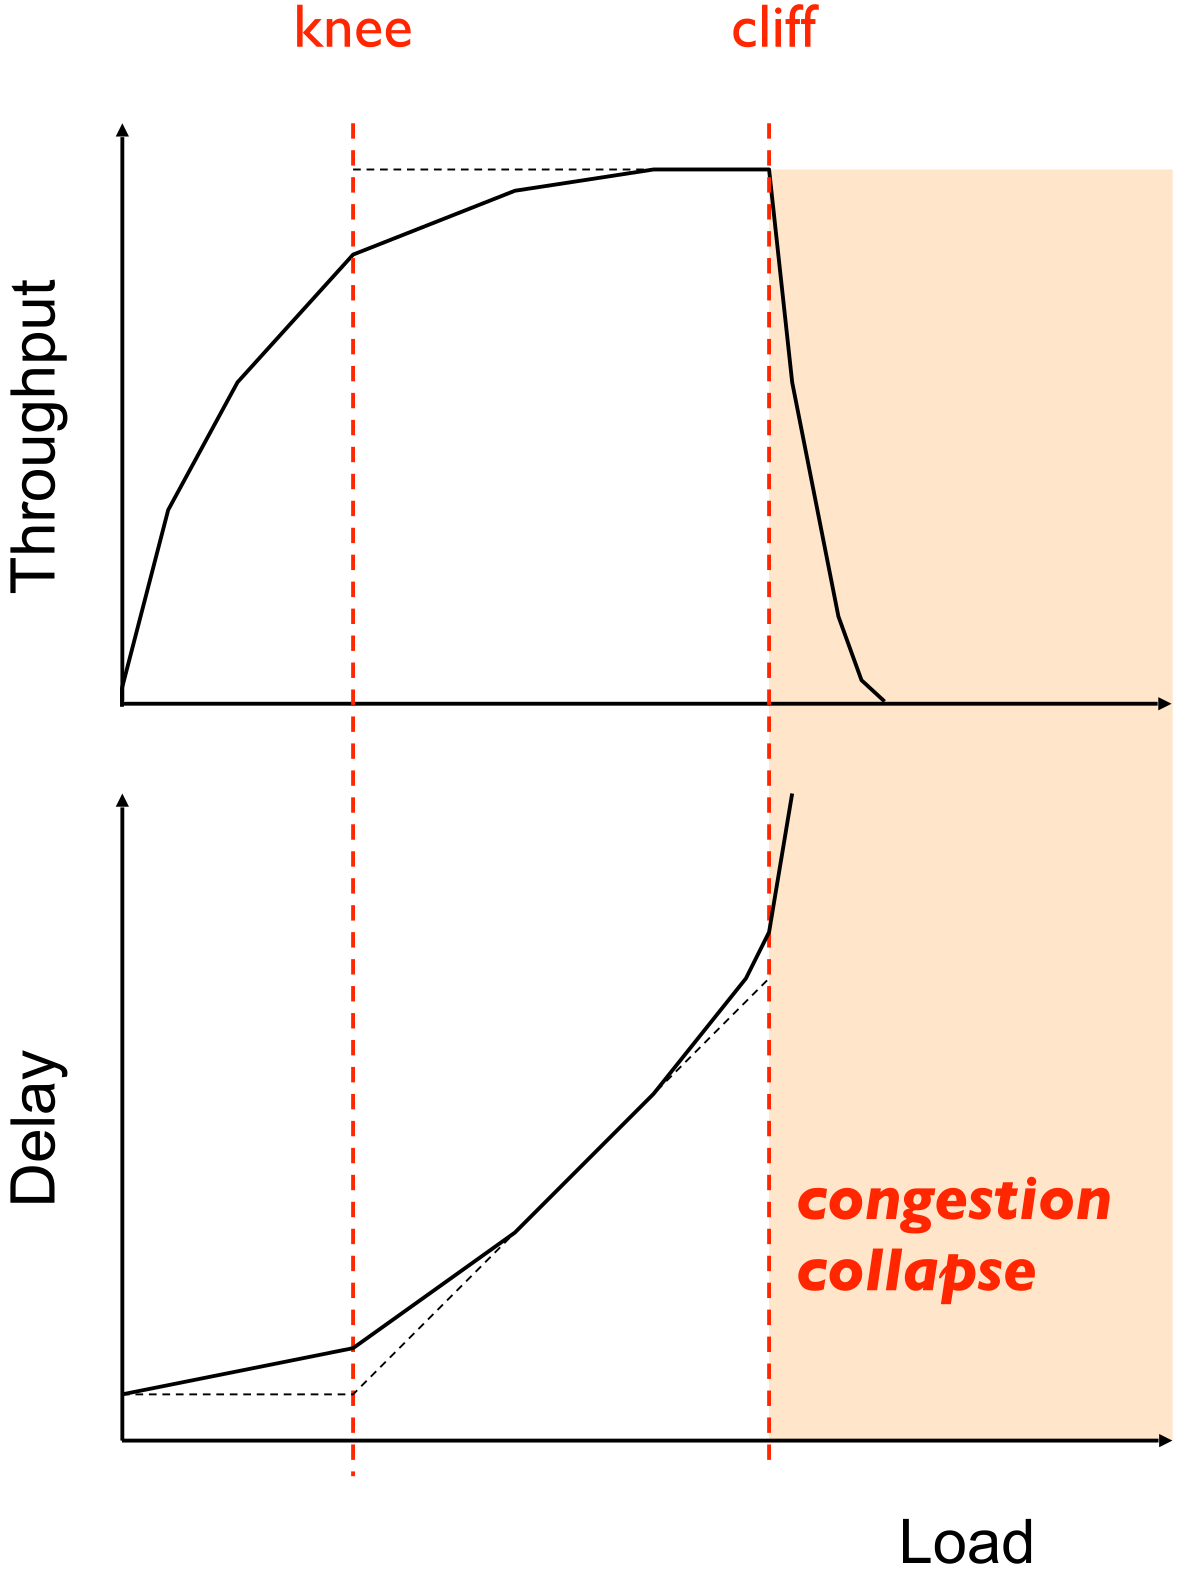
\includegraphics[width=0.6\textwidth]{tcp_congestion.png}
                \end{itemize}
        \end{itemize}
    \item Solves the following:
        \begin{itemize}
            \ides{Bandwidth Estimation:} How to adjust the bandwidth of a single flow to the bottleneck bandwidth?
            \ides{Bandwidth Adaption:} How to adjust the bandwidth of a single flow to variation of the bottleneck bandwidth?
            \ides{Fairness:} How to share bandwidth ``fairly'' among flows?
        \end{itemize}
    \ides{Sender Window}
        \begin{itemize}
            \ides{Receiving Window RWND:} How many bytes can be sent without overflowing receiver buffer
                \begin{itemize}
                    \item Solves flow control problem
                \end{itemize}
            \ides{Congestion Window CWND:} How many bytes can be sent without overflowing the network?
                \begin{itemize}
                    \item Solves congestion control problem
                \end{itemize}
            \ides{Sender Window} $= \min \{\text{CWND}, \text{RWND}\}$
        \end{itemize}
    \ides{Congestion Detection}
        \begin{itemize}
            \item There are multiple approaches
            \ides{Packet Delay:} Measure packet delay
                \begin{itemize}
                    \icon Signal may be noisy
                    \icon Delay varies considerably
                    \icon Hard and risky
                \end{itemize}
            \ides{Packet Loss:} Measure packet loss
                \begin{itemize}
                    \ipro Fail-safe signal
                    \ipro TCP already monitors packet loss
                        \begin{itemize}
                            \ides{Duplicate ACKs:} Mild congestion
                            \ides{Timeout:} Severe congestion
                        \end{itemize}
                \end{itemize}
        \end{itemize}
    \ides{React to Congestion}
        \begin{itemize}
            \item Gently increase window size when not congested, rapidly decrease when congested
            \ides{Slow Start}
                \begin{itemize}
                    \ides{Goal:} Get a quick estimate of the available bandwidth
                    \item Slowly start and the increase exponentially
                    \ides{Initial:} $\text{CWND} = 1$
                    \ides{Upon ACK:} $\text{CWND} = \text{CWND} + 1$
                    \icon Full window may get lost
                \end{itemize}
            \ides{Fairness}
                \begin{itemize}
                    \item Two identical flows should end up with the same bandwidth
                    \item The sum of both flow should be close to the available bandwidth
                        \ides{Trajectory Plot:} We want the bandwidth to be on the intersection of the efficiency and fairness line
                \end{itemize}
            \ides{Additive Increase Multiplicative Decrease (AIMD)}
                \begin{itemize}
                    \ides{Increase:} Add a constant to the point
                        \begin{itemize}
                            \item $(x, y) \to (\alpha + x, \alpha + y)$
                            \item In TCP $\alpha = 1 / \text{CWND}$
                            \item $\implies$ Increment at most by $1$ per RTT
                        \end{itemize}
                    \ides{Decrease:} Take a fraction of the point
                        \begin{itemize}
                            \item In TCP set $\text{CWND} = 1$
                        \end{itemize}
                    \item Converges to fairness and efficiency
                    \item Fluctuates around optimum
                \end{itemize}
            \ides{TCP Congestion Control}
                \begin{itemize}
                    \ides{Slow-Start Threshold (ssthresh):} Threshold which determines switching between slow-start and AIMD
                        \begin{itemize}
                            \ides{Initial:} $\text{ssthresh} = \infty$
                            \ides{On Timeout:} $\text{ssthresh} = \text{cwnd} / 2$
                        \end{itemize}
                    \ides{Fast Recovery}
                        \begin{itemize}
                            \item Reset CWND back to $0$ is wasteful
                            \item Try to react before network gets congested and we get a timeout
                            \item Switch to AIMD
                            \item Done after $3$ consecutive duplicate ACKs
                        \end{itemize}
                    \item Full code:
\begin{verbatim}
Initially:
    cwnd = 1
    sshthresh = infinity

New ACK received:
    if (cwnd < sshthresh):
        # Slow Start
        cwnd = cwnd + 1
    else:
        # AIMD
        cwnd = cwnd + 1 / cwnd
    dup_ack = 0

Timeout:
    # Multiplicative decrease
    sshthresh = cwnd / 2
    cwnd = 1

Duplicate ACKs received:
    dup_ack ++
    if (dup_ack >= 3):
        # Fast recovery
        sshthresh = cwnd / 2
        cwnd = sshthresh
\end{verbatim}
                \end{itemize}
        \end{itemize}
\end{itemize}

\subsubsection{QUIC}
\begin{itemize}
    \item Deployed in 2015 by Google
    \item Has been standardized
    \item Many companies deploy it
    \item Built in many browsers
    \item Belongs to transport, security and application layer
        \begin{itemize}
            \item Builds on top of UDP and is used by HTTP/2 slim
        \end{itemize}
    \item Takes TCP header and puts everything into the UDP date section
    \item Has own congestion control etc.
    \ides{Improvements}
        \begin{itemize}
            \ides{Head Offline Blocking:} One stream fails, stops other stream
                \begin{itemize}
                    \item Sliding window can not continue
                    \item Happens with HTTP/2
                    \item QUIC has multiple streams to prevent that
                \end{itemize}
            \ides{Handshake}
                \begin{itemize}
                    \item TCP handshake is expensive
                        \begin{itemize}
                            \item TCP has $3$-way handshake + $2$-way for TLS
                            \item Total of $3$ RTT or so
                        \end{itemize}
                    \item QUIC needs only one initial handshake
                        \begin{itemize}
                            \item Combines transport and crypto handshake
                        \end{itemize}
                    \ides{O-RTT:} Transport cookie prevents need for handshake if we were connected not long ago
                        \begin{itemize}
                            \item Cookies sent together with the request
                            \ides{Replay Attacks:}
                                \begin{itemize}
                                    \item Server reboot causes the server to not have a knowledge about recently connected clients
                                    \item Clients have to resent request
                                    \item Could cause multiple transactions
                                    \item Nonce (random number) prevents this in TCP
                                        \begin{itemize}
                                            \item This is somehow a challenge
                                            \item A new one is sent which each request
                                        \end{itemize}
                                \end{itemize}
                        \end{itemize}
                \end{itemize}
            \ides{Change of IP}
                \begin{itemize}
                    \item TCP requires source IP to identify a connection
                    \item UDP does not do that
                    \item QUIC adds connectionID to identify a connection
                        \begin{itemize}
                            \item Initialized randomly at handshake
                        \end{itemize}
                \end{itemize}
            \ides{Flow Control}
                \begin{itemize}
                    \item Performed at two levels
                        \ides{Connection Level:} Prevent stream from over-running the receivers buffer
                        \ides{Stream Level:} Prevent individual streams from dominating the connection
                \end{itemize}
            \ides{Evolve TCP}
                \begin{itemize}
                    \item Not really possible
                    \item Dropping certain package attributes looks suspicious and such packets get dropped
                        \begin{itemize}
                            \item Network is conservative
                        \end{itemize}
                \end{itemize}
        \end{itemize}
\end{itemize}

\subsection{Socket}
\begin{itemize}
    \item Application to transport interface
    \item End point of a ``connection''
    \item Two main type of sockets
        \begin{itemize}
            \ides{UDP:} \verb+SOCK_DGRAM+
            \ides{TCP:} \verb+SOCK_STREAM+
        \end{itemize}
    \ides{Port}
        \begin{itemize}
            \item Determine right destination application (demultiplexing) for a packet
            \item 16 bit long
            \item Source port and destination port are carried in the transport header
            \item Different address space for TCP and UDP
            \ides{Well Known Ports:} $0 - 1023$
                \begin{itemize}
                    \item Bound to certain services
                \end{itemize}
            \ides{Ephemeral Ports:} $1024 - 65535$
                \begin{itemize}
                    \item Assigned at random during connection
                \end{itemize}
        \end{itemize}
    \item OS provides mapping:
        \begin{itemize}
            \ides{UDP:} Destination port, destination IP $\leftrightarrow$ socket
            \ides{TCP:} Destination port, destination IP, source port, source IP $\leftrightarrow$ socket
                \begin{itemize}
                    \item Source information needed to identify connection
                \end{itemize}
        \end{itemize}
    \item Protocol, destination port, destination IP uniquely identify a socket
\end{itemize}
